\documentclass[journal]{IEEEtran}
%gambiarra pra alinhar a caption da figura
    \makeatletter
    \long\def\@makecaption#1#2{\ifx\@captype\@IEEEtablestring%
    \footnotesize\begin{center}{\normalfont\footnotesize #1}\\
    {\normalfont\footnotesize\scshape #2}\end{center}%
    \@IEEEtablecaptionsepspace
    \else
    \@IEEEfigurecaptionsepspace
    \setbox\@tempboxa\hbox{\normalfont\footnotesize {#1.}~~ #2}%
    \ifdim \wd\@tempboxa >\hsize%
    \setbox\@tempboxa\hbox{\normalfont\footnotesize {#1.}~~ }%
    \parbox[t]{\hsize}{\normalfont\footnotesize \noindent\unhbox\@tempboxa#2}%
    \else
    \hbox to\hsize{\normalfont\footnotesize\hfil\box\@tempboxa\hfil}\fi\fi}
    \makeatother
%fim da gambi
\usepackage{graphicx}
\usepackage{cite}
\usepackage{mathtools}
\usepackage[section]{placeins}
\usepackage{float}
\usepackage[utf8]{inputenc}
\usepackage[T1]{fontenc}
\usepackage[portuguese]{babel}
\usepackage{hyphenat}
\hyphenation{mate-mática recu-perar}
\usepackage{gensymb}

\begin{document}
\title{Condução de calor unidimensional em uma parede plana por método numérico}
%
%
% author names and IEEE memberships
% note positions of commas and nonbreaking spaces ( ~ ) LaTeX will not break
% a structure at a ~ so this keeps an author's name from being broken across
% two lines.
% use \thanks{} to gain access to the first footnote area
% a separate \thanks must be used for each paragraph as LaTeX2e's \thanks
% was not built to handle multiple paragraphs
%

	\author{\IEEEauthorblockN{Manoel Vieira Coelho Neto 14/0152512\\}
	        \IEEEauthorblockN{Abdullah Zaiter 15/0089392\\}
	        \IEEEauthorblockN{Lukas Lorenz de Andrade  16/0135109\\}
	        \IEEEauthorblockN{Vinícius Félix  13/0145777}}

\maketitle


\section{Introdução}
    Hodiernamente, a aplicação das teorias de transportes - transferência - de calor é infinita, principalmente quando se trata do dimensionamento, simulação, e escolha dos materiais envolvidos no projeto. Assim, é de suma importância o estudo desse campo para a aplicação nos meios industriais, principalmente, de forma a otimizar os processos de fabricação e garantir uma melhor qualidade dos produtos.
    \par Há três principais formas de transmissão de calor, as quais obedecem as Leis da termodinâmica, a saber: condução, convecção e radiação. Na primeira, as moléculas (de mesma massa) interagem por meio de colisões aproximadamente elásticas, trocando energia cinética até que o sistema todo atinja o equilíbrio - a definição de temperatura é justamente a da energia do movimento média das moléculas - ou seja, todas possuírem a mesma quantidade de movimento. Na segunda, há uma combinação da primeira com a dinâmica dos fluidos. Por último, a energia, na forma de onda eletromagnética, é transmitida de um corpo a outro dependendo de várias variáveis, inclusive o fator de forma - modo como se dá a relação entre as superfícies - o qual possibilita calcular a transferência de calor líquida entre os corpos analisados.\cite{comsol}
	\par Dessa forma, todos os fenômenos acima ocorrem devido a uma diferença de temperatura inicial e prosseguem até que esta tenda a zero. Essa energia transferida, calor, é dado no sentido do corpo de maior para o de menor temperatura, de modo que esse fluxo se dá sempre no sentido positivo do eixo coordenado. Ademais, uma forma de atingir o equilíbrio térmico não exclui a outra, de modo que podemos possuir diferentes combinações desses processos.
    \par No entanto, o intuito deste trabalho é a discretização computacional do problema de condução de calor unidimensional em regime transitório com as referidas condições de contorno presentes no roteiro em uma parede. Assim, neste regime, a temperatura não é distribuída de forma uniforme e a condução não é linear com o tempo, mas se aproxima após um $\Delta t\\$. Contudo, a Lei de Fourier e a sua modelação pelas equações diferenciais ordinárias (EDOs) ainda é válida, sendo:
        \begin{align}
            \rho c\frac{\partial T}{\partial t} = \frac{\partial [k \frac{\partial T}{\partial x}]}{\partial x} + \frac{\partial [k \frac{\partial T}{\partial y}]}{\partial y} + \frac{\partial [k \frac{\partial T}{\partial z}]}{\partial z}
        \end{align}
        \par Porém, aplicado a situação em questão e tomando a constante de condutividade “k”  como constante ao longo da estrutura, temos que:
        \begin{quote}
                \begin{itemize}
                    \item condução de calor transiente
                    \begin{align}
                        \rho c\frac{\partial T}{\partial t} = k \frac{\partial ^2T}{\partial t^2}
                    \end{align}\cite[pp. 292]{cengel}
                    \item condução de calor permanente a partir da manipulação de (1)
                    \begin{align}
                        Q' = -k.A\frac{dT}{dx}
                    \end{align}
                    \label{list:proprieties}
                \end{itemize}
            \end{quote}
        
        \par Logo, com base na equação (2), onde '$\rho$’ [$kg/m^3$] é a densidade da estrutura, ‘c’ [J/(kg.ºC)] é a capacidade térmica, T [ºC] a temperatura, será possível a modelação, descrição e simulação computacional do problema proposto.
    \section{Desenvolvimento teórico}
        \par A partir da equação (2) e do método dos elementos finitos e das diferenças finitas pode-se desenvolver aquela a fim de se transformar as EDOs em funções lineares do tempo e espaço, de modo a se calcular a temperatura por iteração sabendo as condições iniciais - condições de contorno. Dessa forma, pelo método das diferenças finitas, podemos aproximar uma derivada por:
        \begin{align}
            f(x+\Delta x) = f(x) + \Delta x \frac{df(x)}{dx} + \frac{1}{2}\Delta x^2\frac{d^2f(x)}{dx} + ...
        \end{align}
        
        \par Tomando $\Delta x$ como muito pequeno (tendendo a zero), pode-se desprezar as frações a partir do terceiro elemento com um erro consideravelmente muito pequeno. Para derivadas de segunda ordem,  aplicando em (4) e adaptando para o problema analisado, temos:
        
        \begin{align}
            \frac{df(x)}{dx} \equiv \frac{f(x + \Delta x - f(x)}{\Delta x}
        \end{align}
        \begin{align}
            \frac{T_{m-1}-2T_m+T_{m+1}}{\Delta x^2}
        \end{align}
        \par Onde Tm  é a temperatura no nó m.
        \par Além do mais, dividimos a superfície em pequenas regiões - quadrados, triângulos, ..., cuja área tende a zero - delimitadas por vértices ou nós (m) e, no caso unidimensional, igual a $\frac{L}{m}$, onde L[m] é a espessura da parede. A medida que $\Delta x$ tende a zero, menor é o erro de T. Passando a equação (6) para o tempo (i) - regime transiente - e aplicando em (2), temos que:
        \begin{multline}
            kA\frac{T_{m-1}-T_m}{\Delta x} + kA\frac{T_{m-1}-T_m}{\Delta x} + \dot{e_m}A\Delta x = \\ \rho A \Delta xc_p\frac{T_{m}^{i+1} - T_{m}^i}{\Delta t}
        \end{multline}\cite[pp.293]{cengel}
        \par Multiplicando a equação acima por $\Delta x$k.A, aplicando o número adimensional de Fourier da malha ($\tau = k.\Delta t \rho.c.\Delta x^2$) e sendo T dependendo do instante de tempo i $\epsilon$ [0,1,2,...], reduz-se a:
		\begin{align}
			T_{m-1}^i - 2T_{m+1}^i + T_{m+1}^i + \frac{\dot{e}_m^i\Delta x^2}{k} = \frac{T_{m}^{i+1}  - T_m^i}{\tau}
		\end{align}
		\par Manipulando e reagrupando os termos em comum chegamos a:
		
        \begin{multline}
        	T_{0}^{i+1} = (1 - 2\tau - 2\tau\frac{h\Delta x}{k})T_{0}^i + 2\tau T_1^i + 2\tau \frac{h\Delta x}{k}\infty + \tau \frac{\dot{e}_0^i\Delta x^2}{k}
        \end{multline}\cite[pp.294]{cengel}
        \par Essa equação relaciona a temperatura em um instante de tempo i+1 com o atual i, de modo que se pode observar a progressão da temperatura no tempo. Porém, caso não haja geração de energia térmica pelo material, o que se aplica ao caso analisado, a condição de estabilidade no limite superior é satisfeita, de modo que $\tau$ = 0.5, a equação acima se resume a:
        \begin{align}
        	T_m^{i+1} = \frac{(T_{m-1}^i + T_{m+1}^i)}{2}
        \end{align}
        A condição que torna a equação (9) estável, ou seja, a teoria não divirja do real, é expressa pela equação (11), que pode ser desenvolvida, aplicando-se perto das condições iniciais e generalizada para toda a estrutura, por (12). Dessa forma, temos: 
      	\begin{align}
      		\tau = \frac{\alpha \Delta t}{\Delta x^2} \leq \frac{1}{2}
      		\\
      		\tau \leq \frac{1}{2(1+h\frac{\Delta x}{k})}
      	\end{align}
      	\par Assim, as equações utilizadas nesse método computacional, são, essencialmente, (9), (10) e (12), sendo (12) igual a $\frac{1}{2}$.
	\section{Simulação}
		\subsection{Problema 1} 
		\par Condução de calor em um só lado (transiente+permanente):
	
		\begin{center}
			T(0, t) = 1\\
			T(1, t) = 0\\
			T(x, 0) = 0
		\end{center}
			
		\begin{figure}[H]
			\begin{center}
				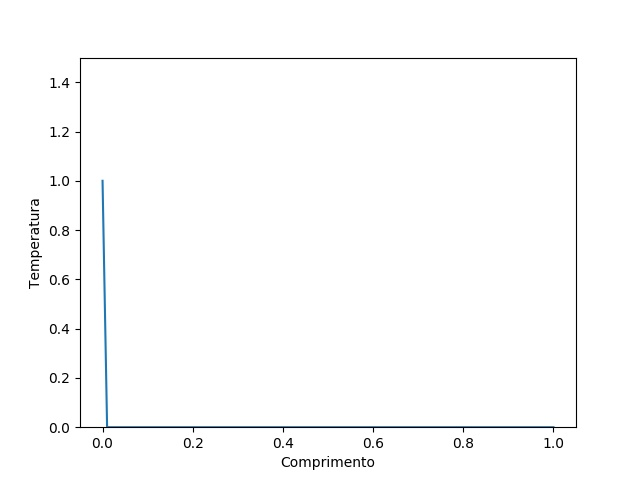
\includegraphics[scale=0.3]{res1-1}
				\caption{Estado inicial (t=0)}
			\end{center}
		\end{figure}
		\begin{figure}[H]
			\begin{center}
				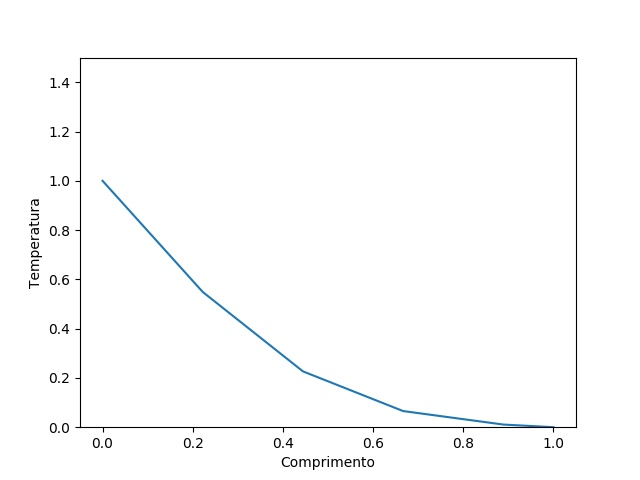
\includegraphics[scale=0.3]{res1-2}
				\caption{Condução no regime transiente}
			\end{center}
		\end{figure}
		\begin{figure}[H]
			\begin{center}
				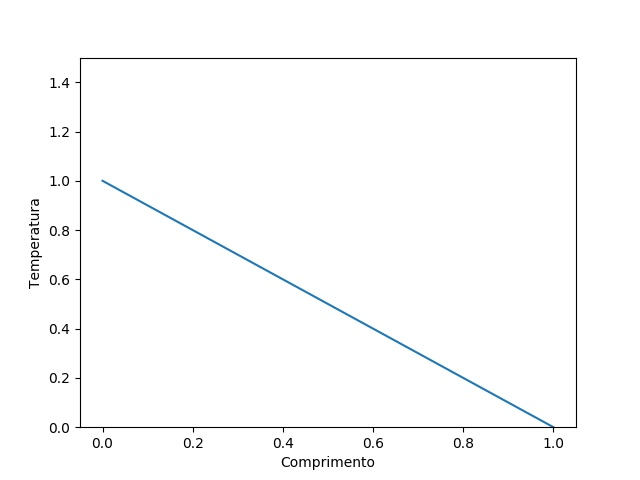
\includegraphics[scale=0.3]{res1-3}
				\caption{Condução no regime permanente (equilíbrio térmico)}
			\end{center}
		\end{figure}
		\par Para o caso 1 é possível observar no decorrer do tempo $t$ como o a curva se comporta em regime transiente até que passe ao regime permanente e tenda para uma reta, em uma distribuição de calor linear.
	\subsection{Problema 2}
		\par Condução de calor no sentido de ambos os lados (temperatura distribuída no início + equilíbrio térmico):
		\begin{center}
			T(0, t) = 0\\
			T(1, t) = 0\\
			T(x, 0) = 1
		\end{center}
		\begin{figure}[H]
			\begin{center}
				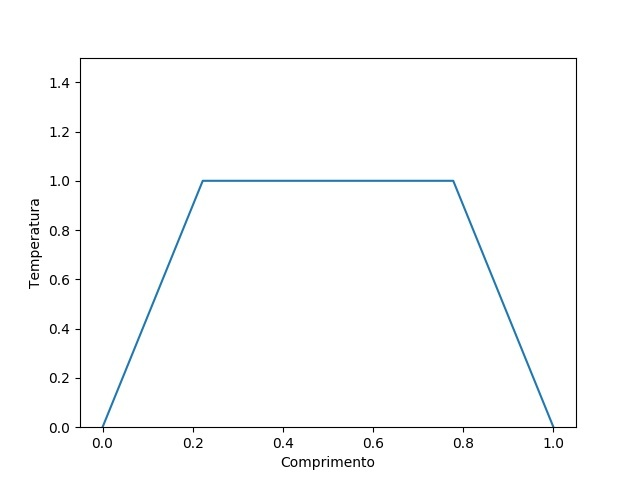
\includegraphics[scale=0.3]{res2-1}
				\caption{Estado inicial (t=0)}
			\end{center}
		\end{figure}
		\begin{figure}[H]
			\begin{center}
				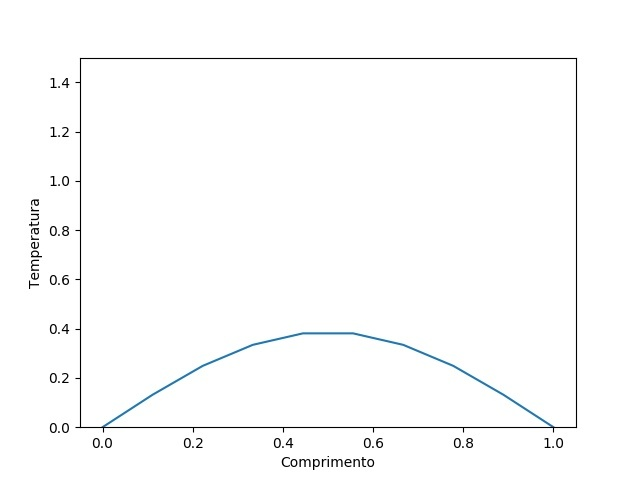
\includegraphics[scale=0.3]{res2-2}
				\caption{Condução no regime transiente}
			\end{center}
		\end{figure}
		\begin{figure}[H]
			\begin{center}
				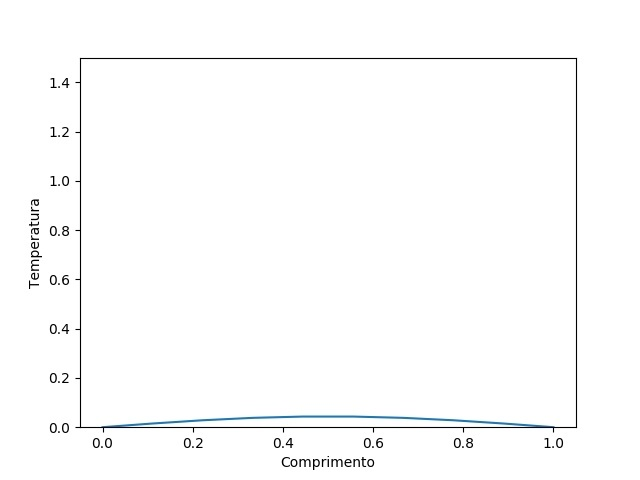
\includegraphics[scale=0.3]{res2-3}
				\caption{Condução no regime permanente (equilíbrio térmico)}
			\end{center}
		\end{figure}
		No caso 2, ambas as pontas da barra estão em 0$^{\circ}C$ e a temperatura ao longo da barra é igual a 1$^{\circ}C$ e assim co o decorrer o tempo o calor tende a se distribuir na barra até que esta esteja na temperatura das pontas em uma distribuição linear e constante igual a 0.
        
\section{Resultados e Conclusão}
    A partir das figuras 1 a 3 percebe-se o comportamento da temperatura ao longo da espessura genérica da parede no primeiro problema analisado. A figura 1 faz menção ao início do processo de troca de calor por condução onde a troca ocorre num regime transiente (representada por uma função exponencial decrescente).
    \par Também é notório nas figuras 4 a 6 o comportamento da temperatura ao longo da espessura genérica da parede no segundo problema analisado. Onde a parede troca calor com o ambiente dos dois lados, onde na figura 4 a temperatura está máxima e tende para diminuir pelo efeito da troca de calor com o ambiente que tem uma temperatura menor, essa temperatura vai descendo à medida que o tempo tende a infinito até atingir a temperatura do ambiente como mostrado na figura 6. O comportamento do decrescimento da temperatura nas figuras 4 a 6 no regime transiente até o permanente é explicado fisicamente pois a parede esfria de fora para dentro onde a parte que tem contato direto com o ambiente esfria mais rápido do que a parte de dentro da parede.
	\par Traçando um paralelo entre as análises numéricas e algébricas podemos concluir que em regime permanente as curvas traçadas obtém aproximações com grande acurácia em relação aos valores reais, tendo seu momento transitório,referente a valores de $t$ antes da total convergência, comportamento esperado pelo embasamento teórico. 
    

\bibliographystyle{IEEEtran}

\bibliography{exemplo}



\end{document}
